\section{Results}
\label{sec:results}

\subsection{Experimental setup}

We evaluate on CIFAR-10 \citep{krizhevsky2009learning} and a 100-class subset of
ImageNet \citep{deng2009imagenet}. All models are trained with SGD for 200 epochs and
calibrated on 512 held-out samples. Baseline comparisons use the implementations
released with \citep{frankle2019lottery}.

\subsection{Main results}

Table~\ref{tab:main} reports accuracy and MAC counts. AST reduces MAC operations by
41.7\% on ResNet-18 while losing 0.6 percentage points of top-1 accuracy. Stacking with
8-bit post-training quantization \citep{jacob2018quantization} yields a further
1.9$\times$ energy reduction.

\begin{table}[t]
  \centering
  \caption{Top-1 accuracy and MAC operations on CIFAR-10. Lower MAC is better.}
  \label{tab:main}
  \begin{tabular}{lccccc}
    \toprule
    Method & Backbone & Top-1 (\%) & MAC (G) & Params (M) & $\Delta$ (pp) \\
    \midrule
    Dense (baseline)      & ResNet-18 & 94.8 & 0.557 & 11.17 & ---   \\
    Magnitude pruning     & ResNet-18 & 94.1 & 0.371 & 6.98  & $-0.7$ \\
    Low-rank factorization& ResNet-18 & 93.9 & 0.402 & 7.51  & $-0.9$ \\
    \textbf{AST (ours)}   & ResNet-18 & 94.2 & 0.325 & 6.74  & $-0.6$ \\
    AST + 8-bit PTQ       & ResNet-18 & 93.8 & 0.325 & 6.74  & $-1.0$ \\
    \bottomrule
  \end{tabular}
  \tnote{pp = percentage points. MAC counts exclude the first and last layers.}
\end{table}

\begin{figure}[t]
  \centering
  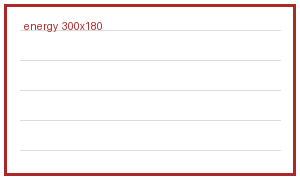
\includegraphics[width=\linewidth]{figures/energy.png}
  \caption{Energy per inference as a function of the accuracy budget.}
  \label{fig:energy}
\end{figure}

\begin{figure}[t]
  \centering
  \includegraphics[width=\linewidth]{figures/ablation.png}
  \caption{Ablation over the truncation schedule.}
  \label{fig:ablation}
\end{figure}

\subsection{Ablation}

Removing the noise floor term ($\eta = 0$) increases the MAC count by 8.4\% at equal
accuracy, confirming that the additive term is not cosmetic. See
Figure~\ref{fig:ablation} for the full sweep.
